\documentclass[10pt, tikz, border=5pt]{standalone}

\usetikzlibrary{positioning}
\usetikzlibrary{shadows}
\usetikzlibrary{fit, backgrounds}
\usetikzlibrary{shapes.multipart}
\usetikzlibrary{3d}


\tikzset{
    ionode/.style={draw, circle, minimum size=0.5cm},
    layer/.style={
        draw, rectangle, rounded corners, minimum width=3cm, minimum height=0.5cm, align=center
    },
    convblock/.style={layer, copy shadow, fill=gray!20!white},
    fc/.style={layer, rectangle split, rectangle split parts=2},
    conv/.style={layer, copy shadow, fill=gray!20!white},
    flow/.style={->, ultra thick}
}

\begin{document}

% node distace=1cm
% could also use node labels and label rotation

\begin{tikzpicture}[node distance=0.5cm, font=\small]
	\begin{scope}[node distance=0.2cm]

		\begin{scope}[node distance=0.1cm]
			\node[layer, minimum width=2cm, rectangle split, rectangle split parts=4] (cbconv) {
				\nodepart{one}
				Conv3D\\
				$5 \times (3 \times 3 \times 3)$
				\nodepart{two}
				BatchNorm3D
				\nodepart{three}
				MaxPool3D\\
				$2 \times 2 \times 2$
				\nodepart{four}
				ReLU
			};
			\node[align=center, above=of cbconv] (cbname) {Conv3D Block\\$5 @ 5\times60\times50$};
			%\node[right=of cbconv] (cbnamepos) {};
			%\node[rotate=-90, align=center, anchor=south] (cbname) at (cbnamepos) {ConvBlock 3D\\$5 @ 5\times60\times50$};
		\end{scope}

		\begin{scope}[on background layer]
			\node[convblock, dashed, fit={(cbconv) (cbname)}] (cb1) {};
		\end{scope}

		\node[convblock, below=of cb1.south] (cb2) {Conv3D Block\\$5 @ 25 \times 30 \times 25$};

		% \draw[flow] (cb1.south) -- node[right] {$5 \times 50 \times 60 \times 50$} (cb2.north);

		\node[convblock, below=of cb2.south] (cb3) {Conv3D Block\\$5@12 \times 15 \times 12$};

		% \draw[flow] (cb2.south) -- node[right] {$5 \times 25 \times 30 \times 25$} (cb3.north);

		\node[fc, below=of cb3.south] (fc1) {Linear ($64$) \nodepart{two} ReLU};

		% \draw[flow] (cb3.south) -- node[right] {$5 \times 12 \times 15 \times 12$} (fc1.north);

		\node[fc, below=of fc1.south] (fc2) {Linear ($32$) \nodepart{two} ReLU};

		% draw fully connected - maybe a bit cluttered?
		\iffalse
			\foreach \sanchor in {south west, south, south east} {
					\foreach \nanchor in {north west, north, north east} {
							\draw (fc1.\sanchor) -- (fc2.\nanchor);
						}
				}

			%\draw (fc1.south) -- node[draw, rectangle, fill=white] {$64$} (fc2.north);
		\fi

		%\draw[flow, ultra thick] (fc1.south) -- node[right] {$64$} (fc2.north);

		\node[fc, below=of fc2.south] (fc3) {Linear ($2$) \nodepart{two} Softmax};

		%\draw[flow] (fc2.south) -- node[right] {$64$} (fc3.north);

	\end{scope}
	\node[ionode, label=above:$100 \times 120\times 100$, above=of cb1] (input) {};

	\node[above=of input.north] (mri) {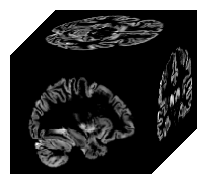
\includegraphics[angle=-90]{mri-cube.pdf}};

	\iffalse
		\node[above=3.5cm of input.north] (mriorigin) {};
		\begin{scope}[rotate around z=-90, shift={(mriorigin)}, inner sep=0, outer sep=0]
			\def\cubelen{2cm}
			\node[canvas is xz plane at y=1, anchor=west] {\includegraphics[width=\cubelen, angle=-90]{axial.png}};
			\node[canvas is xy plane at z=1, anchor=west, inner sep=0] {\includegraphics[height=\cubelen]{sagittal.png}};
			\node[canvas is zy plane at x=0] {\includegraphics[height=\cubelen]{coronal.png}};
			%\node[above=of input, canvas is zy plane at x=0] {\includegraphics{coronal.png}};
		\end{scope}
	\fi

	%\draw[flow] (input.south) -- node[right] {$100 \times 120 \times 100$} (cb1.north);
	\draw[flow] (input.south) -- (cb1.north);
	\node[below=of fc3.south] (output) {};

	\node[ionode, fill=blue!20, label=below:CN, below left=of output, inner sep=0] (outputcn) {-};
	%\node[rotate=-90, below=of outputcn, anchor=center] {CN};

	\node[ionode, fill=red!20, label=below:AD, below right=of output,inner sep=0] (outputad) {+};
	%\node[rotate=-90, below=of outputad, anchor=center] {AD};

	\draw[flow] (fc3.south) -- (output.center) -| (outputcn);
	\draw[flow] (fc3.south) -- (output.center) -| (outputad);
\end{tikzpicture}

\end{document}